 
An artificial neural network is a network of connected units called neurons or perceptrons, each arc which connects two neurons $i$ and $j$ is associated with a weight $w_{ji}$. Perceptrons share the some
structure for all models, what really define the model in the family is how the perceptrons are arrange and how are they conneceted, for example if there are cycles or not.
As you can see in figure \ref{neuron_model} each neuron is \textit{fed} with a set inputs which are the weighted outputs of other neurons. Formally the output of a perceptron $\phi_j$
is defined as:
 
\begin{align}
&\phi_j \triangleq \sigma(a_j)\\
&a_j \triangleq \sum_l w_{jl}\phi_l +b_j
\end{align}

where $w_{jl}$ is the weight of the connection between neuron $l$ and neuron $j$, $\sigma(\cdot)$ is a non linear function and $b_j \in \mathbb{R}$ is called bias.


\tikzstyle{nn_style}=[->,shorten >=1pt,auto,node distance=1.5cm,
  thick,
  neuron/.style={circle,fill=white!50,node distance=1cm,draw,minimum size=0.7cm,font=\sffamily\normalsize},
  missing/.style={circle,font=\sffamily\Large,node distance=0.95cm},
  label/.style={node distance=1.2cm,rectangle,fill=white!50,draw=none,minimum size=0.7cm,font=\sffamily\normalsize},
  layer/.style={rectangle,fill=white!50,draw,minimum width=1.5cm,font=\sffamily\Large},
  loopStyle/.style={in=120,out=60, distance=2.5cm},
  weight/.style = {above,sloped,pos=0.3},]
\begin{figure}
 \centering
\begin{tikzpicture}[nn_style]

  \node[neuron]    (x0)       {};
  \node[neuron]    (x1)[below of=x0]   {};
  \node[neuron]    (x2)[below of=x1]   {};
  \node[missing]   (x3)[below of=x2]   {$\vdots$};
  \node[neuron]    (xn)[below of=x3]   {};
  
  
  \node[label]    (u0)[left of=x0]   {$\phi_0$};
  \node[label]    (u1)[left of=x1]   {$\phi_1$};
  \node[label]    (u2)[left of=x2]   {$\phi_2$};
  \node[label]    (un)[left of=xn]   {$\phi_n$};
  
  
  \node[layer] (hl)[ right of=x2,node distance=3.5cm] {$\Sigma$};
  \node[neuron](bias)[above of=hl,node distance=2cm]{$1$};
  \node[layer] (ol)[right of=hl,node distance=2.5cm] {$\sigma$};
  
  \node[label]  (phi)[right of=ol,node distance=2cm] {$\phi_j$};
   
  
  \path[->] (x0) edge [] node[weight]{$w_{0j}$}   (hl)
	    (x1) edge [] node[weight]{$w_{1j}$}   (hl)
	    (x2) edge [] node[weight]{$w_{2j}$}   (hl)
	    (xn) edge [] node[weight]{$w_{nj}$}   (hl)
 	    (bias) edge[]  node[]{$b_{j}$}(hl)
	    (u0) edge []   (x0)
	    (u1) edge []   (x1)
	    (u2) edge []   (x2)
	    (un) edge []   (xn)
	    (hl) edge []   node[]{$a_{j}$}(ol)
	    (ol) edge []   (phi);

\end{tikzpicture}
\caption{Neuron model}
\label{neuron_model}
\end{figure}


A neural network looks like the one in figure \ref{fully_connected}

\tikzstyle{nn_style}=[->,shorten >=1pt,auto,node distance=1.5cm,
  thick,
  neuron/.style={circle,fill=white!50,node distance=2.5cm,draw,minimum size=0.7cm,font=\sffamily\normalsize},
  missing/.style={circle,font=\sffamily\Large,node distance=0.95cm},
  label/.style={node distance=1.2cm,rectangle,fill=white!50,draw=none,minimum size=0.7cm,font=\sffamily\normalsize},
  layer/.style={rectangle,fill=white!50,draw,minimum width=1.5cm,font=\sffamily\Large},
  loopStyle/.style={in=120,out=60, distance=2.5cm},
  weight/.style = {above,sloped,pos=0.3},]
\begin{figure}
 \centering
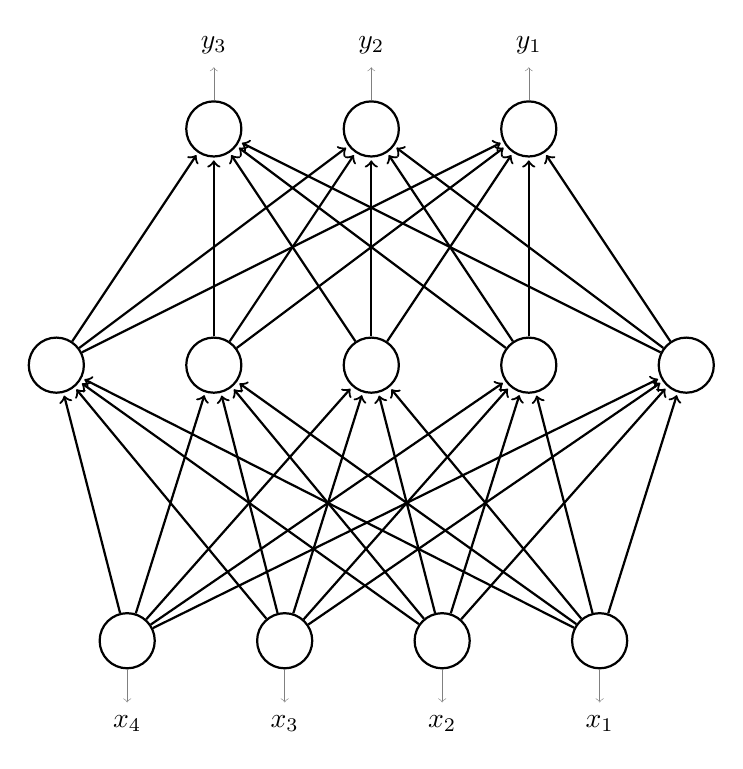
\begin{tikzpicture}[nn_style]
   
   \def\layersep{3cm}
  
    % Draw the input layer nodes
    \foreach \name / \y in {1,...,4}
    % This is the same as writing \foreach \name / \y in {1/1,2/2,3/3,4/4}
        \node[neuron, pin=below:$x_\y$] (I-\name) at (-\y *2,0) {};

    % Draw the hidden layer nodes
    \foreach \name / \y in {1,...,5}
        \path[yshift=0.5cm]
            node[neuron] (H-\name) at (-\y *2  + 1.1, \layersep) {};

    % Draw the output layer nodes
    \foreach \name / \y in {1,...,3}
        \path[yshift=0.5cm]
            node[neuron, pin=above:$y_\y$] (O-\name) at (-\y *2 - 0.9, \layersep*2) {};

    % Connect every node in the input layer with every node in the
    % hidden layer.
    \foreach \source in {1,...,4}
        \foreach \dest in {1,...,5}
            \path (I-\source) edge (H-\dest);
            
    % Connect every node in the hidden layer with every node in the
    % output layer.
    \foreach \source in {1,...,5}
        \foreach \dest in {1,...,3}
            \path (H-\source) edge (O-\dest);

\end{tikzpicture}
\caption{Artificial neural network example}
\label{fully_connected}
\end{figure}


It sometime useful to think of a neurual network as series of layers, one on top of each other, as depicted in figure \ref{layered_nnet}. The first layer is called the input layer and its units are \textit{fed}
with external inputs, the upper layers are called \textit{hidden layers} because their's outputs are not observed from outside except the last one which is called \textit{output layer} because it's output 
is the output of the net.

Whene we describe a network in this way is also useful to adopt a different notation: we describe the weights of the net with a set of matrixes $W_i$ one for each layer, and neurons are no more
linearly indexed, insted with refer to a neuron with a relative index with respect to the layer; this allows to write easier equations in matrix notation
\footnote{In the rest of the book we will refer to the latter notation as \textsl{matrix notation} and to the previous one as \textsl{linear notation}}.


\tikzstyle{rnn_style}=[->,shorten >=1pt,auto,node distance=1.5cm,
  thick,
  neuron/.style={circle,fill=white!50,draw,minimum size=0.7cm,font=\sffamily\Large\bfseries},
  missing/.style={circle,fill=white!50,draw=none,minimum size=0.7cm,font=\sffamily\Huge\bfseries},
  label/.style={node distance=1.2cm,rectangle,fill=white!50,draw=none,minimum size=0.7cm,font=\sffamily\normalsize},
  layer/.style={rectangle,fill=white!50,draw,minimum width=4cm,font=\sffamily\normalsize},
  loopStyle/.style={in=120,out=60, distance=2.5cm},]
\begin{figure}
 \centering
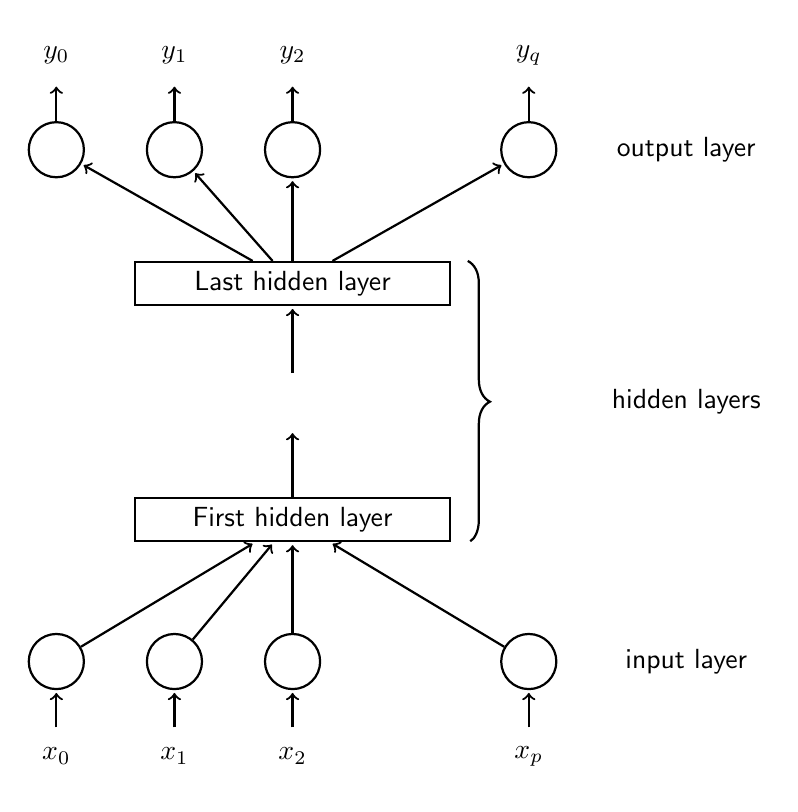
\begin{tikzpicture}[rnn_style]

  \node[neuron]    (x0)       {};
  \node[neuron]    (x1)[right of=x0]   {};
  \node[neuron]    (x2)[right of=x1]   {};
  \node[missing]   (x3)[right of=x2]   { $\hdots$};
  \node[neuron]    (xn)[right of=x3]   {};
  
  \node[label]    (u0)[below of=x0]   {$x_0$};
  \node[label]    (u1)[below of=x1]   {$x_1$};
  \node[label]    (u2)[below of=x2]   {$x_2$};
  \node[label]    (un)[below of=xn]   {$x_p$};
  
  

    
  \node[layer] (hl)[above of=x2,node distance=1.8cm] {First hidden layer};
  \node[missing] (hls)[above of=hl,node distance=1.5cm]{$\hdots$};
  \node[layer] (ol)[above of=hls,node distance=1.5cm] {Last hidden layer};
  
  \draw[decorate,decoration={brace,raise=6pt,amplitude=8pt}, thick,-]
   (ol.north east)--(hl.south east);



  
  \node[neuron] (o1) at (0,6.5) {};
  \node[neuron] (o2)[right of=o1] {};
  \node[neuron] (o3)[right of=o2] {};
  \node[missing](o4)[right of=o3] {$\hdots$};
  \node[neuron] (on)[right of=o4] {};
  
  
  \node[label]    (y0)[above of=o1]   {$y_0$};
  \node[label]    (y1)[above of=o2]   {$y_1$};
  \node[label]    (y2)[above of=o3]   {$y_2$};
  \node[label]    (yn)[above of=on]   {$y_q$};
  
     
  \node[label]    (hls_label)[right of=hls,node distance=5cm]   {hidden layers};
  \node[label]    (input_label)[right of=xn,node distance=2cm]   {input layer};
  \node[label]    (output_label)[right of=on,node distance=2cm]   {output layer};
  
  
  \path[->] (x0) edge [] node[]{}   (hl)
	    (x2) edge []   (hl)
	    (x1) edge []   (hl)
	    (xn) edge []   (hl)
	    (u0) edge []   (x0)
	    (u1) edge []   (x1)
	    (u2) edge []   (x2)
	    (un) edge []   (xn)
	    (ol) edge []   (o1)
	    (ol) edge []   (o2)
	    (ol) edge []   (o3)
	    (ol) edge []   (on)
	    (o1) edge []   (y0)
	    (o2) edge []   (y1)
	    (o3) edge []   (y2)
	    (on) edge []   (yn)
	    (hl) edge []  node[]{} (hls)
	    (hls) edge []  node[]{} (ol);


\end{tikzpicture}
\caption{Layered structure of an artificial neural network}
\label{layered_nnet}
\end{figure}